\documentclass[border=10pt]{standalone}
\usepackage{amsmath}
\usepackage{pgfplots}
\usepgfplotslibrary{fillbetween}
\pgfplotsset{compat=1.18}
\begin{document}
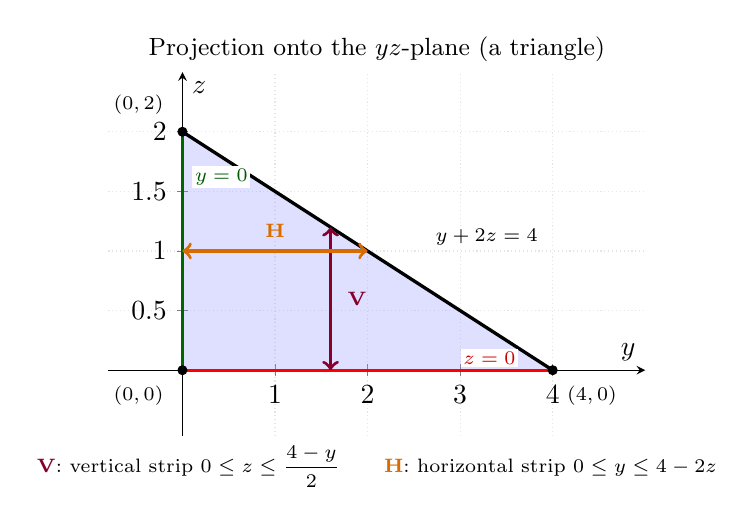
\begin{tikzpicture}
\begin{axis}[width=8.4cm, height=6.2cm, axis lines=middle,
    xlabel={$y$}, ylabel={$z$}, xmin=-0.8,xmax=5.0, ymin=-0.55,ymax=2.5,
    xtick={1,2,3,4}, ytick={0.5,1,1.5,2},
    grid=major, grid style={gray!20,densely dotted}]
  \addplot[name path=PL, blue!45, opacity=0, domain=0:4, samples=2] {(4-x)/2};
  \addplot[name path=AX, blue!45, opacity=0, domain=0:4, samples=2] {0};
  \addplot[fill=blue!45, opacity=0.28] fill between[of=PL and AX];
  \addplot[very thick, domain=0:4, samples=2] {(4-x)/2};
  \node[font=\scriptsize, anchor=south west, fill=white, inner sep=1pt] at (axis cs:2.7,1.02) {$y+2z=4$};
  \addplot[red, very thick, domain=0:4, samples=2] {0};
  \draw[green!40!black, very thick] (axis cs:0,0) -- (axis cs:0,2);
  \node[font=\scriptsize, text=green!35!black, anchor=west, fill=white, inner sep=1pt] at (axis cs:0.1,1.62) {$y=0$};
  \node[font=\scriptsize, text=red!80!black, anchor=west, fill=white, inner sep=1pt] at (axis cs:3.0,0.10) {$z=0$};

  \draw[<->, purple!70!black, very thick] (axis cs:1.6,0) -- (axis cs:1.6,1.2);
  \node[font=\scriptsize\bfseries, text=purple!70!black, anchor=west] at (axis cs:1.68,0.6) {V};
  \draw[<->, orange!85!black, very thick] (axis cs:0,1.0) -- (axis cs:2.0,1.0);
  \node[font=\scriptsize\bfseries, text=orange!85!black, anchor=south] at (axis cs:1.0,1.03) {H};

  \addplot[only marks, mark=*, mark size=1.6] coordinates {(0,0) (4,0) (0,2)};
  \node[font=\scriptsize, anchor=north east] at (axis cs:-0.1,-0.05) {$(0,0)$};
  \node[font=\scriptsize, anchor=north west] at (axis cs:4.05,-0.05) {$(4,0)$};
  \node[font=\scriptsize, anchor=south east] at (axis cs:-0.1,2.06) {$(0,2)$};
\end{axis}
\node[font=\small, align=center, anchor=south] at (current bounding box.north) {Projection onto the $yz$-plane (a triangle)};
\node[font=\scriptsize, align=left, anchor=north] at (current bounding box.south)
  {\textcolor{purple!70!black}{\textbf{V}}: vertical strip $0\le z\le\dfrac{4-y}{2}$\qquad
   \textcolor{orange!85!black}{\textbf{H}}: horizontal strip $0\le y\le 4-2z$};
\end{tikzpicture}
\end{document}
